\documentclass[compress,handout,10pt]{beamer}

\newlength{\wideitemsep}
\setlength{\wideitemsep}{\itemsep}
\addtolength{\wideitemsep}{100pt}
\let\olditem\item
\renewcommand{\item}{\setlength{\itemsep}{0.5\baselineskip}\olditem}

\usetheme{Singapore}
\usecolortheme{rose}
\usefonttheme[onlymath]{serif}

\usepackage{float}
\floatstyle{boxed}
\usepackage{epsfig}
\usepackage{colortbl}
\usepackage{mathpazo}
\usepackage{graphicx}
\usepackage{movie15}
\usepackage{bm}
\usepackage{verbatim}
\usepackage{comment}
\usepackage{caption}
\usepackage{subcaption}
\usepackage{graphicx}
\graphicspath{{extra/}}
\captionsetup[subfigure]{labelformat=empty}
\captionsetup[figure]{labelformat=empty}

\newcommand{\mygreen}{\color{green!50!black}}
\newcommand{\myblue}{\color{blue}}
\newcommand{\myred}{\color{red}}
\newcommand{\mycolor}{\color{red}{c}\color{blue}{o}\color{green}{l}\color{orange}{o}\color{cyan}{r}}
\newcommand{\mysize}{\scriptsize{s}\small{i}\normalsize{z}\Large{e}}
\newcommand{\myshape}{\textcircled{s}\textit{h}\texttt{a}\textsf{p}\textsc{e}}

\title{\\
{\color{black} \bf {\Large Constructing Dedicated Portfolio \\against District Bond Obligations \\from a Simplified Scenario}\newline \\
 } }
\subtitle{{\color{black} \bf{\underline{Blackrock} }\\ \vspace{2mm}\small \bf{Sponsor:}} \\\vspace{2mm}  \color{black} Stone \& Youngberg } 
\author{  {\bf{Participants:}} \\ \vspace{2mm}
Zhenhan Zhao, Shihong Li\\
\vspace{2mm} 

\includegraphics[width=0.25\textwidth]{jhu.png} 
} 
\institute{JHU AMS 2012 FALL}



\begin{document}

\begin{frame}[plain]
    \titlepage
\end{frame}

\begin{frame}
    \frametitle{Outline}
   \begin{itemize}
    \item Introduction 
    \item Problem Statement
        \item Technical Background 
\item Analysis
   \item Results
    \item conclusions
   \end{itemize}
\end{frame}

\section{Introduction}

\begin{frame}
    \frametitle{My sponsor}
\begin{itemize}
\item  Stone \& Youngberg\\

\includegraphics[width=0.28\textwidth]{stone.jpeg}\\
\vspace{4mm}
A division of Stifel Nicolaus\\ 
\vspace{3mm}
Leader in municipal finance in the Far West, roots in California dating back to 1931\\
\vspace{3mm}
Work with state and local governments, school districts and non-profit agencies to strengthen local communities.  

\end{itemize}
\end{frame}

\begin{frame}
    \frametitle{Background}
Poway Unified School District is a school district located in Poway, California.\\
\vspace{3mm}
It borrowed 105 million dollars from investors by selling a district bond.\\
Taxpayers in the area will end up with 1 billion billl. \\
\vspace{3mm}
Taxpayers in the Poway district will have to start paying about 50 million a year to cover the bill
\end{frame}


\begin{frame}
    \frametitle{Problems and Objective}
\underline{ \bf{\large {Problems}}}\\
\vspace{3mm}
Authorized more taxes from taxpayers $\rightarrow$ break down the promises to the community Poway  $\rightarrow$ decided to seek help from Stone \& Youngberg \\
\vspace{3mm}
S\&Y came up with a strategy to construct a portfolio to satisfy future financial obligations\\
\vspace{8mm}

\underline{ \bf{\large {Objective}}}\\
\vspace{3mm}
Try to select the appropriate assets at a minimum cost and  maximum matching degree , then find the optimal asset proportion


\end{frame}

\section{Technical Background}

\begin{frame}
    \frametitle{Technical Approaches}
\begin{itemize}
\item Polynomial regression $\rightarrow$ the present value of the liability stream\\
\item Pick a series of assets that are suitable $\rightarrow$ satisfy the  district future financial obligation\\
\item Iimmunization strategy  $\rightarrow$ make sure the portfolio  matches both the duration and convexity 
\end{itemize}
\end{frame}


\section{Analysis}
\begin {frame}
\frametitle{Analysis Scheme}
\begin{enumerate}[step 1]
    \item Conducted intensive research into bond obligations. Generated a complete analysis about the payment periods, cash flows, bond features, and etc..\\
\vspace{5mm}
    \item Computed the present value of the liability stream with polynomial regression  \\
.
\end{enumerate}
\end{frame}

\begin {frame}
\frametitle{Analysis Scheme}
\begin{enumerate}
    \item[step 3] Searched the financial market for reliable capital assets based on credit risk, interest rate risk, and payment matching. Found 32 assests.\\
  \vspace{5mm}
   \item[step 4] Set up a linear program to decide the weight of each bond.\\
\end{enumerate}
\end{frame}

\begin {frame}
\frametitle{Analysis Scheme}
\begin{enumerate}[step 1]

    \item[step 5] Used the immunization strategy to make sure the portfolio  matches both the duration and convexity of the liabilities.\\
\vspace{5mm}
    \item[step 6] Carried out scenario anaylsis and sensitive analysis to examine the validity of our research.
\end{enumerate}
\end{frame}


\begin{frame}
    \frametitle{Dummy Data}
\begin{table}[h]
\centering  
\begin{tabular}{cccc}
\hline
Date  &Liability  &Date  &Liability\\ \hline  
7/15/2012  &6  &7/15/2016  &8\\
1/15/2013  &6  &1/15/2017  &8\\ 
7/15/2013  &9  &7/15/2017  &8\\ 
1/15/2014  &9  &1/15/2018  &8\\ 
7/15/2014  &10 &7/15/2018  &6\\ 
1/15/2015  &10  &1/15/2019  &6\\ 
7/15/2015  &10  &7/15/2019  &5 \\ 
1/15/2016  &10  &1/15/2020  &5\\ \hline
\end{tabular}
\caption{Liability Stream.}
\end{table}
\end{frame}

\begin{frame}
    \frametitle{Calculating present value of the liability stream}
\begin{itemize}
\item Polynomial \\
\vspace{1mm}
We used seven yield rates between 6 months and 10 years, 3rd order polynomial curve 
\begin{figure}[bottom]
    \begin{center}
        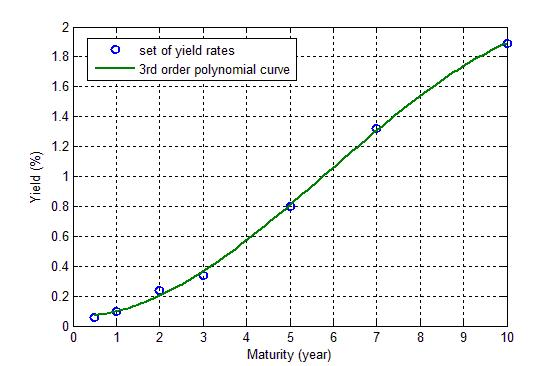
\includegraphics[width=6cm,height=4.5cm]{fit.jpg}
    \end{center}
    \caption{fit}
    \label{figure1}
\end{figure}
\end{itemize}
\end{frame}

\begin{frame}
    \frametitle{Calculating present value of the liability stream}
\begin{itemize}
\item Bootstrapping \\
First we compute the discount factor. The basic idea of bootstrapping is like this,\\
\begin{eqnarray}
  \ P &=& C(t_1) \times d(t_1) + C(t_2) \times d(t_2)
\end{eqnarray}

Once we have d(t1), from the equation, we will get d(t1) and d(t2), etc. After we compute the discount factors, we compute the present value of each liability .
\end{itemize}
\end{frame}

\begin{frame}
    \frametitle{Calculating present value of the liability stream}
\begin{table}[h]
\centering  
\begin{tabular}{ccccc}
\hline
Date  &Liability  &PV from Polynomial  &PV from Bootstrap\\ \hline  
7/15/2012  &6    &6.00                        &6.00                      \\
1/15/2013  &6    &5.99                      &5.99                  \\
7/15/2013  &9  &8.98                        &8.98                     \\
1/15/2014  &9  &8.96                       &8.96                     \\
7/15/2014  &10 &9.93                        &9.93                      \\
1/15/2015  &10 &9.89                        &9.90                     \\
7/15/2015  &10  &9.84                        &9.86                    \\
1/15/2016  &10  &9.77                        &9.79                      \\
7/15/2016  &8        &7.76                        &7.76                     \\                             
1/15/2017  &8      &7.68                        &7.68                     \\
7/15/2017  &8       &7.60                       &7.59                      \\
1/15/2018  &8       &7.51                       &7.49                     \\
7/15/2018  &6    &5.56                        &5.55                     \\ 
1/15/2019  &6      &5.48                       &5.47                     \\ 
7/15/2019  &5      &4.50                        &4.49                      \\ 
1/15/2020  &5       &4.43                       &4.43                      \\ \hline
sum       &124           &119.9                    &119.86

\end{tabular}
\caption{Liability Stream.}
\end{table}
\end{frame}

\begin{frame}
    \frametitle{Asset Allocation}
We will choose around 30 assets to construct a portfolio. The assets are a pool of Treasury notes with different maturities. \\
\vspace{3mm}
Reasons:\\
\vspace{3mm}
\begin{itemize}
\item Credit Risk \\
Governmental bonds ensures that all obligations will be fulfilled without concerned of default risks. 
\end{itemize}
\end{frame}

\begin{frame}
    \frametitle{Asset Allocation}
\begin{itemize}
\item Interest Risk \\
We choose bonds with fixed payments to eliminate TIPS
\vspace{8mm}
\item Payment Matching\\
Our assets should pay semi-annually. We choose T-notes with maturity BEFORE the exact payment dates. 
\end{itemize}
\end{frame}

\begin{frame}
    \frametitle{Asset Allocation}
\begin{table}[h]
\centering  
\begin{tabular}[width=4cm,height=2.3cm]{ccc}
\hline
T-NOTE 30/06/12  &T-NOTE 30/11/14       &T-NOTE  31/05/17\\
T-NOTE 15/07/12   &T-NOTE 31/12/14        &T-NOTE 30/06/17\\
T-NOTE31/12/12   &T-NOTE  31/05/15   &T-NOTE 30/11/17\\
T-NOTE 15/01/13    &T-NOTE 30/06/15  & T-NOTE 31/12/17\\
T-NOTE 30/06/13  & T-NOTE 30/11/15   &T-BOND  31/05/18\\
T-NOTE 15/07/13    &T-NOTE 31/12/15   &T-NOTE  31/05/18\\
T-NOTE 15/12013   &T-NOTE 31/05/16   &T-BOND 15/11/18\\
T-NOTE 31/12/13  & T-NOTE 30/06/16   &T-NOTE 15/11/18\\
T-NOTE 31/05014   &T-NOTE 30/11/16   &U S TREAS SEC 15/05/19\\
T-NOTE 30/06/14   &T-NOTE 31/1216  &T-NOTE 15/05/19\\
                                                &&U S TREAS SEC 15/11/19\\\hline
\end{tabular}
\caption{Assets}
\end{table}
\end{frame}

\begin{frame}
\frametitle{Immunization}
Goal: A linear programming system  that by changing the weight of  bonds  and excess cash from each period,  initial investment and the excess cash will be minimized.\\
\end{frame}

\begin{frame}
\frametitle{Immunization}
Two Constraints: \\
\vspace{5mm}
\noindent $\bullet$ All expected cash flow from the bond portfolio must exceed the expected liability in the same period.\\
\vspace{3mm}
$\bullet$ All the weights of the bonds in the portfolio must be positive.  \\
\end{frame}

\begin{frame}
\frametitle{Some definitions....}
Duration 
\begin{align}
D=-\dfrac {1} {p}\left[-\dfrac {1} {1+y}+y^{\ast }\sum t^{\ast }\dfrac {C_{t}} {\left( 1+y\right) ^{t}}\right]
\end{align}
Convexity
\begin{align}
C=\dfrac {1} {(1+y}t^{\ast }\sum t\ast \left( t+1\right) \dfrac {C_{t}} {\left( 1+y\right) ^{t}\cdot p}
\end{align}
\end{frame}

\begin{frame}
\frametitle{Immunization}
\vspace{8pt}
The linear program is set up as follows:\\
\vspace{5mm}
\noindent $\bullet$ Minimize total price of the bond portfolio\\
\vspace{3mm}
\noindent $\bullet$ Change non-negative quantity (or weight) of each bond\\
\vspace{3mm}
\noindent $\bullet$ Subject to: duration, convexity and present value of the bond portfolio are equal to those of the liability stream.\\
\end{frame}

\begin{frame}
\begin{table}[h]
\centering  
\begin{tabular}{cccc}
\hline
Feature  &Amount\\ \hline  
Total Price  &113.2814 million dollars\\
Total Duration  &7.85432\\ 
Total Convexity  &86.74968\\ 
Total PV  &119.8625 million dollars\\ 
\hline
\end{tabular}
\caption{Bond Portfolio	}
\end{table}
\vspace{4mm}
\centering Minimized initial cost = 112.21 million dollars.\\
\end{frame}


\section{Results}
\begin{frame}
    \frametitle{Sensitivity analysis}
\begin{figure}[htb]
  \begin{center}
      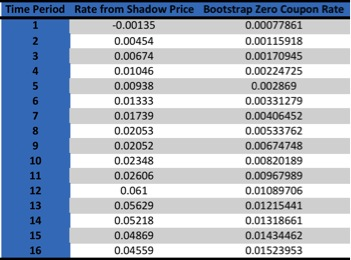
\includegraphics[width=0.7\textwidth]
{cf.jpg}
    \end{center}
    \caption{Cash Flow Matching Portfolio}
\end{figure}
\end{frame}

\section{Conclustions}
\begin{frame}
    \frametitle{Conclusions}
The portfolio price, 113.28 million dollars, slightly higher\\
\vspace{3mm}
(If relax this constraint a little, say, maximally 5 in the red every month \\ $\rightarrow$ will still reach a CLOSE SOLUTION )\\
\vspace{12mm}
\begin{itemize}
\item[*]Conclusion: that our solution is ROBUST, and the fundamental challenge lies in the SCREENING of the bonds.
\end{itemize}
\end{frame}


\begin{frame}
\Huge\centerline {Thanks for Watching!}
\end{frame}

\end{document}